%!TEX root = ../thesis.tex
\newchap{Theoretical framework}\label{sec:TH}
\minitoc
\section{The Standard Model of particle physics}

The Standard Model of particle physics (SM) is a quantum field theory (QFT) that describes all the fundamental forces known beside gravity: the electromagnetic, the strong and the weak force. \\
A QFT is a framework that combines quantum mechanics, classical field theory and special relativity, allowing us to describe a particle as the excitation of a quantum field or, more formally, with an irreducible representation of the Poisson group that is characterized by its mass, spin, and additional quantum numbers.
Such theories are characterized by a Lagrangian density $\Lg{}$ that must be Lorentz invariant, must respect locality and must be renormalizable, \ie the perturbative expansions of the amplitudes must converge. \\
In the SM, additional local symmetries (Gauge symmetries) are imposed to describe the interactions between particles and for each (global) symmetry, according to the Noether theorem \cite{NoetherInvarianteVariationsprobleme}, a conserved charge arises.

\subsubsection*{Particles of the Standard Model}
Particles are divided into two main categories: fermions and bosons. 
Fermions are particles with half integer spin that obey to the Fermi-Dirac statistics and to the Pauli principle. 
Furthermore, each fermion has an antiparticle with the same mass but opposite quantum numbers.\\
Bosons are particles with integer spin that obey the Bose-Einstein statistics. In the SM there are the vector bosons (spin 1), the mediators of the forces, and the Higgs boson, the only scalar boson of the SM (spin 0). All the particles of the SM and their properties are summarized in \Fig{fig:SMpart}.



\begin{figure}[h!]
    \centering
    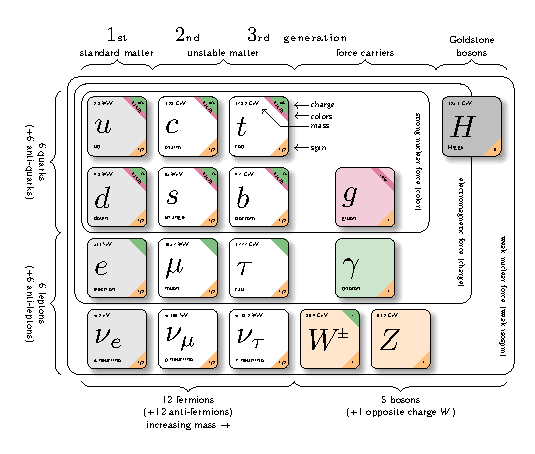
\includegraphics[width=1\linewidth]{fig/chap02-theory/SMpart.pdf}
    \caption{Fundamental particles of the Standard Model \cite{BurgardCarstenStandardExample}}
    \label{fig:SMpart}
\end{figure}

%commented
\iffalse
\paragraph*{Interactions}
The three fundamental interactions described by the SM are the electromagnetic, the strong and the weak force.\\
Each interaction has a Gauge boson that arises from a symmetry group.\\
The \emph{electromagnetic interaction} is described by the quantum electrodynamics (QED) \cite{FeynmanQED:Matter}, a \U{1} Gauge theory, and is mediated by the photon.\\
The \emph{strong interaction} is described by the quantum chromodynamics (QCD) \cite{Chromodynamics1995QUANTUMCHROMODYNAMICS} through the \SU{3} group.\\

\fi

\paragraph*{Fermions}
Fermions are divided into leptons and quarks and are divided in 3 generations for a total of 12 fermions.\\
\emph{Quarks} are the constituents of the hadrons. They have a fractional electric charge and a color charge (and an anticolor charge for the antiquarks).\\
Quarks are divided into up-type quarks (up, charm, and top) with an electric charge of $Q=2/3$ and into down-type quarks (down, strange and bottom) with an electric charge of $Q=-1/3$.
One of the main properties of the QCD is the color confinement: isolated particles must be color singlets, so free quarks can't be observed because they hadronize (see sec. \ref{sub:QCD}).
The only exception is the top quark that decays before the hadronization due to its short lifetime.\\
Furthermore, weak interactions don't couple identically with all the flavours, but down-type quarks flavour are mixed according to the CKM matrix as explained in the section \ADDREF.\\
\emph{Leptons} are the electron (\Pe), the muon (\PGm), the tau (\PGt) and their respective neutrinos (\PGne, \PGnGm, \PGnGt).
A charged lepton and its respective neutrino represent a generation of leptons with a corresponding family lepton flavor number $L_{\ell_i}=n_{\ell_i}-n_{\PAl_i}$ that, in SM, is conserved together with the total lepton number $L=n_\ell-n_\PAl$.
The leptons participate in all the interactions except the strong force.\\


\subsection{Gauge theories and the QED}\label{sub:gauge_qed}
\paragraph*{Fermion free fields}
The Lagrangian (density) for a free fermion field is the Dirac Lagrangian
\begin{equation}\label{eq:Dirac}
\mathcal{L}_{\text{Dirac}}=i\bar{\psi}\gamma^{\mu}\partial_{\mu}\psi-m\bar{\psi}\psi
\end{equation}
where $\aff{\psi}{}=\ff{\psi}{}^\dagger\gamma^0$ is the adjoint Dirac spinor, and $\gamma^\mu$ are the 4 Dirac matrices that obey the Clifford algebra $\{\gamma^\mu,\gamma^\nu\}=2\eta^{\mu\nu}$\\
The corresponding equation of motion has two solutions: the one with the positive energy represents the fermion field, the one with the negative energy represents the anti-fermion field.\\
\paragraph*{Gauge theories}
The standard procedure to introduce a global symmetry in the Lagrangian and a Gauge boson field is the following:
\begin{enumerate}
    \item Introduce a local symmetry based on a Lie group:
    \begin{equation}\label{eq:spinor_gauge}
        \psi(x) \to \psi^\prime (x)=g(x) \psi(x) = e^{i \alpha_a(x) t^a}\psi(x)
    \end{equation}
    where $g(x)$ is a representation of the group and $t^a$ its generators
    \item Replace the partial derivatives $\partial_\mu$ with the covariant derivative $D_\mu$
    \begin{equation}\label{eq:covariant_derivative}
        D_{\mu}\psi(x)=\left(\partial_{\mu}-i g\,A_{\mu}^{a}(x)\,t^{a}\right)\psi(x)\;
    \end{equation}
    where $g$ is the coupling constant between the fermion field and the gauge fields and $A^a_\mu$ the Gauge fields 
    \item The covariant derivative should transform according to the gauge group $D_\mu \psi(x)\to g(x) D_\mu \psi(x)g^\dagger (x)$ and, with some calculation, it is possible to find that the Gauge filed transform as the following under the action of the Gauge group
    \begin{equation}\label{eq:gauge_field_transformation}
        A_{\mu}(a)\rightarrow g(x)\left(A_{\mu}(x)+\frac i g\,\partial_{\mu}\right)\,g^{\dagger}(x)
    \end{equation}
    where $A_\mu=A_\mu^a(x)t^a$
    \item The final Lagrangian now has a global invariance for the Gauge group and for the Noether Theorem there is a conserved charge. Furthermore, in this procedure, another vector massless field arises.
\end{enumerate}
\paragraph*{Quantum electrodynamics}
The simplest case of a Gauge theory is the quantum electrodynamics (QED) in which the Gauge group is \U{1}, a commutative group for which holds $g(x)g(y)=g(y)g(x)$\\
The fundamental representation of the \U{1} group is $g(x)=e^{i \alpha(x)}$, \ie a local phase.\\
Imposing the \U{1} invariance on the Dirac Lagrangian (\Eq{eq:Dirac}), we obtain the QED Lagrangian (\Eq{eq:QED}).\\
In the SM, all the fermions, except the neutrinos, have an electric charge and are involved in the electromagnetic interaction.
\begin{equation}\label{eq:QED}
    \Lg{QED}=i\bar{\psi}\gamma^{\mu}(\partial_{\mu}+i q A_{\mu})\psi-m\bar{\psi}\psi-\frac{1}{4}F^{\mu\nu}F_{\mu\nu}
\end{equation}
where $A_\mu$ is the photon field, $q$ the elementary electron charge and $F_{\mu\nu}=\partial_\mu A_\nu-\partial_\nu A_\mu$ the electromagnetic tensor \\


\subsection{Quantum chromodynamics}\label{sub:QCD}
The quantum chromodynamics (QCD) is the \SU{3} Gauge theory that describes the strong interaction and involves gluons and quarks, bonding together into hadronic states.
The quantum number related to strong interaction in the color charge.
Applying the gauging technique described in the section \ref{sub:gauge_qed} is possible to obtain the QCD Lagrangian.
\begin{equation}\label{eq:QCD}
    \Lg{QCD}=i\bar{\psi}\gamma^{\mu}\partial_{\mu}\psi-m\bar{\psi}\psi-i g_{s}\bar{\psi}\gamma^{\mu}\lambda_{a}\psi G_{a,\mu}-\frac{1}{4}G_{a}^{\mu\nu}G_{a,\mu\nu}
\end{equation}
where \(G_{\mu\nu}^{a}=\partial_{\mu}G_{\nu}^{a}-\partial_{\nu}G_{\mu}^{a}-g_{s}f^{a b c}G_{\mu}^{b}G_{\nu}^{c}\) is the corresponding of the electromagnetic tensor for the strong force, $\lambda_a$ are the \SU{3} generators, and $f^{abc}$ the \SU{3} structure constants\\
Each quark carries a color charge and each quark an anticolor charge and, since \SU{3} has 8 generators, 8 gluons exist (or just one gluon that can carry one of 8 couples of color-anticolor).\\
There are significant differences with the QED to the non-abelianity of \SU{3}:
\begin{itemize}
    \item \textbf{Gluon self-coupling}: gluons can interact with each other.
    \item \textbf{Asymptotic freedom}: the coupling strength decreases with the energy, \ie at large energy scales the quarks become quasi-free.\\
    The coupling constant of the strong interaction depends on the energy scale \cite{Deur2016TheCoupling}
    \begin{equation}\label{eq:alphas_run}
        \alpha_S(\mu^2)\propto \frac{1}{\ln \left( \frac{\mu^2}{\Lambda_{\text{QCD}}^2}\right)}        
    \end{equation}
    Where $\Lambda_{QCD}\approx 200 \MeV$ and $\mu$ is the energy scale.\\
    When $\mu \gg \Lambda_{QCD}$, strong interactions can be described using perturbative techniques (pQCD) but, at low-energy scales, the QCD is non perturbative and that leads to the third property of the QCD
    \item \textbf{Color confinement}: At low-energy scales, the strong coupling is so large that quarks are always bounded in color singlets and isolated quarks can't be observed.\\
    This is also why the strong force has a limited range, while the electromagnetic force has an infinite range.
\end{itemize}

\subsection{Electroweak unification}
\paragraph*{Weak interactions}
The weak interaction was first introduced by Enrico Fermi to explain the $\beta$ decay through the 4 point Fermi interaction \ADDREF and is the only force that involves all the fermions and that violates the parity and the charge parity conservation. \\
The quantum number related to the weak interaction is the weak Isospin, generated by the \SU{2} gauge group that creates 3 gauge bosons: the $W^+$, the $W^-$ and the $Z$ boson.\\
Trying to build the weak Lagrangian only using the gauging technique described in the section \ref{sub:gauge_qed} in this case doesn't work for different reasons:
\begin{itemize}
    \item The W boson and the Z boson would have the same coupling to the fermions, while this is experimentally wrong. To address this problem, the weak interaction was unified to the electromagnetic interaction.
    \item The W/Z bosons are proven to be massive bosons, while gauge bosons are always massless. The massive term can't be added arbitrary to the Lagrangian because such a theory would be non renormalizable \ADDREF \\
    Masses have to be added through the Higgs mechanism as described in the section \ref{sub:SM}
    \item The Weak interaction doesn't couple identically with all the quarks, but the flavours are mixed by the Cabibbo-Kobayashi-Maskawa (CKM) matrix \ADDREF as described in section \ref{sec:CKM}. The elements of the CKM matrix are complex, and this leads to the CP violation.
    \item To introduce the parity violation in the Lagrangian, the $\gamma^\mu$ in the interaction term of the Lagrangian has to be replaced with $\gamma^\mu \left(1-\gamma^5 \right)/2 $.\\
    The term $(1-\gamma^5)/2$ is the left chirality projector, and this implies that weak interaction couples only with the left part of the spinor. This will turn to be true only for charged weak interactions, while for neutral weak interactions, the mixing between the photon and the Z boson in the electroweak (EW) unification process will reintroduce the coupling with the right spinors.
\end{itemize}

\paragraph*{Electroweak unification}\label{sub:EW}
The electromagnetic and weak interactions were unified in the Glashow-Weinberg-Salam theory \ADDREF based on the $\SU{2} \bigotimes \U(1)$ symmetry group.


\subsection{The Standard Model}\label{sub:SM}
\paragraph*{The Higgs mechanism and the spontaneous symmetry breaking}

\section{The CKM matrix}\label{sec:CKM}
\subsection{The $V_{cb}$ element}

\subsection{Measurement of $|V_{cb}|$ with B mesons semileptonic decays}

\paragraph*{Inclusive measurement}

\paragraph*{Exclusive measurement}


\section{The Top quark}
\subsection{Top pairs production at an hadron collider}
\paragraph*{Extra jets}
\subsection{Top quark decay}
\subsection{Measurement of $|V_{cb}|$ with top pairs semileptonic decays}